%%%%%%%%%%  Start of 7 element lattice section  %%%%%%%%%%%%%%%%%%

%%% THIS IS THE SIZE OF LATTICE POINTS %%%
%\newcommand{\dotsize}{.8pt}

\frame[label=results]{
  \frametitle{Are all lattices with at most 7 elements representable?}
  %{\color{gray}As of February 2011...}
             {\it As of Spring 2011...}

             \vspace{-.5cm}

             \begin{center}
               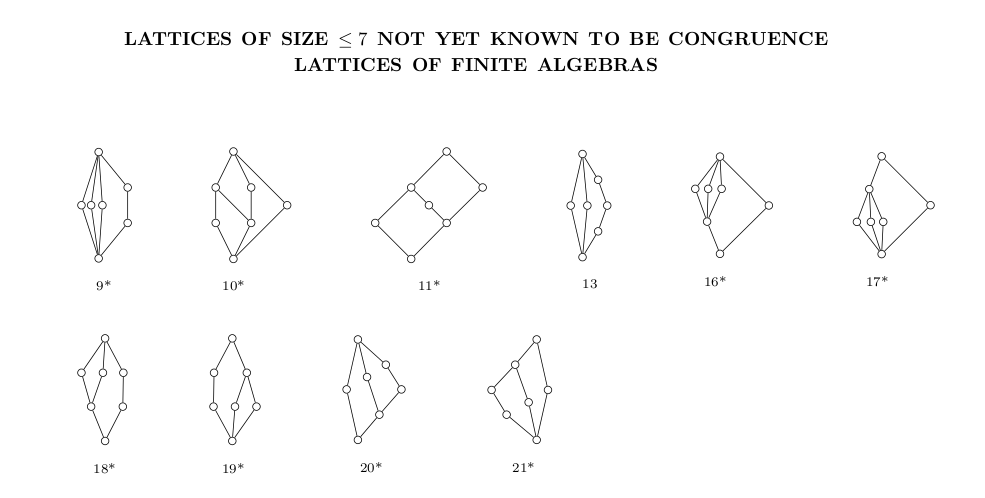
\includegraphics[height=2.3in]{figures/Sevens}
             \end{center}
             \hfill {\small {\it Figure courtesy of Peter Jipsen.}}
}  


\begin{frame}[label=knownresults,shrink=5]{
    Are all lattices with at most 7 elements representable?}

  \begin{columns}
    \begin{column}{0.2\textwidth}
      \begin{center}
        \begin{tikzpicture}[scale=.5]

          % L19
        \node (bottom) at (0,0)  [draw, circle, inner sep=\dotsize] {};
        \node (top) at (0,3)  [draw, circle, inner sep=\dotsize] {};
        \node (11) at (1,1)  [draw, circle, inner sep=\dotsize] {};
        \node (n11) at (-1,1)  [draw, circle, inner sep=\dotsize] {};
        \node (12) at (1,2)  [draw, circle, inner sep=\dotsize] {};
        \node (n12) at (-1,2)  [draw, circle, inner sep=\dotsize] {};
        \node (01) at (0,1)  [draw, circle, inner sep=\dotsize] {};

        \draw[semithick] (bottom) to (11) to (12) to (top) to (n12) to (n11) to (bottom) to (01) to (12);

          \draw (0,-1) node {$L_{19}$};
          \visible<2->{ {\color{red}\draw[font=\large] (1,-.6) node{$\text{\rlap{$\checkmark$}}$ };}
            %\draw[font=\large] (2.5,-.6) node { {\footnotesize Jipsen}};
          }

        \end{tikzpicture}
      \end{center}
    \end{column}
    \begin{column}{0.2\textwidth}
      \begin{center}
        \begin{tikzpicture}[scale=.4]
          % L20
      \foreach \j in {0,...,4}
      {
        \node (0\j) at (0,\j)  [draw, circle, inner sep=\dotsize] {};
      }
      \node (152) at (1.5,2)  [draw, circle, inner sep=\dotsize] {};
      \node (n125) at (-1,2.5)  [draw, circle, inner sep=\dotsize] {};
      \draw[semithick] (01) to (02) to (03) to (04) to (n125) to (01) to (00) to (152) to (04);

          \draw (0,-1) node {$L_{20}$};
          \visible<2->{        {\color{red}\draw[font=\large] (1,-.6) node{$\text{\rlap{$\checkmark$}}$ };}
            %\draw[font=\large] (3,-.6) node { {\footnotesize Jipsen}};
          }
        \end{tikzpicture}
      \end{center}
    \end{column}
  \end{columns}

  \begin{columns}
    \begin{column}{0.2\textwidth}
      \begin{center}
        \begin{tikzpicture}[scale=.4]

          
        \node (bottom) at (0,0)  [draw, circle, inner sep=\dotsize] {};
        \node (top) at (0,5)  [draw, circle, inner sep=\dotsize] {};
        \node (n115) at (-1,1.5)  [draw, circle, inner sep=\dotsize] {};
        \node (015) at (0,1.5)  [draw, circle, inner sep=\dotsize] {};
        \node (115) at (1,1.5)  [draw, circle, inner sep=\dotsize] {};
        \node (n252) at (-2.5,2)  [draw, circle, inner sep=\dotsize] {};
        \node (03) at (0,3)  [draw, circle, inner sep=\dotsize] {};
        \draw[semithick] 
        (bottom) to (n252) to (top)
        (bottom) to (n115) to (03) to (115) to
        (bottom) to (015) to (03) to (top);
       %\draw (-4.5,2.2) node {$L \cong$};



          \draw (0,-1) node {$L_{17}$};
        \end{tikzpicture}
      \end{center}
    \end{column}

    \begin{column}{0.2\textwidth}
      \begin{center}
        \begin{tikzpicture}[scale=.5]

          %\newcommand{\dotsize}{1};
\node[lat] (0) at (0,0) {};
\node[lat] (1) at (-0,1) {};
\node[lat] (2) at (1,2) {};
\node[lat] (3) at (-1,2) {};
\node[lat] (4) at (-0,2) {};
\node[lat] (5) at (-0,3) {};
\node[lat] (6) at (-0,4) {};
%\draw[font=\scriptsize] (0,-.5) node {[A4, (C2 x C2 x C2 x C2) : A5]};
%\draw[font=\scriptsize] (0,-1) node {SmallGroup(960,11358) Index 80};

\draw[semithick]
(0) to (1) to (4) to (5) to (6)
(0) to (2) to (6) to (3) to (0);


          \draw (0,-.6) node {$L_{13}$};

        \end{tikzpicture}
      \end{center}
    \end{column}

    \begin{column}{0.2\textwidth}
      \begin{center}
        \begin{tikzpicture}[scale=.3]

          % L11 aka L3 
        \node (bottom) at (0,0)  [draw, circle, inner sep=\dotsize] {};
        \node (top) at (2,6)  [draw, circle, inner sep=\dotsize] {};
        \node (n22) at (-2,2)  [draw, circle, inner sep=\dotsize] {};
        \node (22) at (2,2)  [draw, circle, inner sep=\dotsize] {};
        \node (13) at (1,3)  [draw, circle, inner sep=\dotsize] {};
        \node (04) at (0,4)  [draw, circle, inner sep=\dotsize] {};
        \node (44) at (4,4)  [draw, circle, inner sep=\dotsize] {};

        \draw[semithick] (bottom) to (22) to (44) to (top) to (04) to (13) to (22)
        (bottom) to (n22) to (04);
  
          \draw (1,-1) node {$L_{11}$};
          %{$L_{11}$ {\small (aka $L_3$)}};

        \end{tikzpicture}
      \end{center}
    \end{column}

  \end{columns}


  \begin{columns}

    \begin{column}{0.2\textwidth}
      \begin{center}
        \begin{tikzpicture}[scale=.5]

          %% ``L9'' is the pentegon with two extra wings.
      \foreach \j in {0,3} 
      { \node (7\j) at (6.5,\j)  [draw, circle, inner sep=\dotsize] {};}
      \node (71) at (7,1.5)  [draw, circle, inner sep=\dotsize] {};
      \node (61) at (6,1.5)  [draw, circle, inner sep=\dotsize] {};
      \node (51) at (5,1.5)  [draw, circle, inner sep=\dotsize] {};
      \foreach \j in {1,2} 
      { \node (8\j) at (7.8,\j)  [draw, circle, inner sep=\dotsize] {};}
      \draw[semithick] (70) to (51) to (73) to (61) to (70) to (71) to (73) to
      (82) to (81) to (70);
      

          \draw (6.5,-1) node {$L_{9}$};

        \end{tikzpicture}
      \end{center}
    \end{column}


    \begin{column}{0.2\textwidth}
      \begin{center}
        \begin{tikzpicture}[scale=.5]

          %%  The elusive winged-2x3 %%
      \node (01) at (0,1)  [draw, circle, inner sep=\dotsize] {};
      \foreach \j in {0,2} 
      { \node (1\j) at (1,\j)  [draw, circle, inner sep=\dotsize] {};}

      \foreach \j in {1,3} 
      { \node (2\j) at (2,\j)  [draw, circle, inner sep=\dotsize] {};}
      { \node (32) at (3,2)  [draw, circle, inner sep=\dotsize] {};}
      \draw[semithick] (10) to (01) to (12) to (23) to (32) to (21) to (10) (21) to (12);
      { \node (m11) at (-1,1)  [draw, circle, inner sep=\dotsize] {};}
      \draw[semithick] (10) to (m11) to (23);


          \draw (1,-.8) node {$L_{10}$};

        \end{tikzpicture}
      \end{center}
    \end{column}
  \end{columns}
\end{frame}


\begin{frame}[label=knownresults,shrink=5]{Finding representations...}
  \framesubtitle{...as intervals in subgroup lattices}

  \begin{columns}
    \begin{column}{0.2\textwidth}
      \begin{center}
        \begin{tikzpicture}[scale=.4]

          
        \node (bottom) at (0,0)  [draw, circle, inner sep=\dotsize] {};
        \node (top) at (0,5)  [draw, circle, inner sep=\dotsize] {};
        \node (n115) at (-1,1.5)  [draw, circle, inner sep=\dotsize] {};
        \node (015) at (0,1.5)  [draw, circle, inner sep=\dotsize] {};
        \node (115) at (1,1.5)  [draw, circle, inner sep=\dotsize] {};
        \node (n252) at (-2.5,2)  [draw, circle, inner sep=\dotsize] {};
        \node (03) at (0,3)  [draw, circle, inner sep=\dotsize] {};
        \draw[semithick] 
        (bottom) to (n252) to (top)
        (bottom) to (n115) to (03) to (115) to
        (bottom) to (015) to (03) to (top);
       %\draw (-4.5,2.2) node {$L \cong$};




          \draw (-2,4) node {$L_{17}$};
          \uncover<2->{
            \draw[font=\scriptsize] (0.3,5.5) node {$G$};
            \draw[font=\scriptsize] (0.3,-.4) node { $H$};
            \draw[font=\scriptsize] (0,-1.3) node {{\tt SmallGroup(288,1025)}};
            \draw[font=\scriptsize] (0,-2.2) node { $|G:H|=48$};
          }

        \end{tikzpicture}
      \end{center}
    \end{column}

    \uncover<2->{
      \begin{column}{0.6\textwidth}
        \begin{itemize}
        \item 
          The group $G = (A_4 \times A_4) \rtimes C_2$ has a subgroup $H\cong S_3$ such
          that $\lb H,G \rb\cong L_{17}$.
          \vskip10pt
        \item<2-> ...so the dual $L_{16}$ is also representable.
          %% \\[8pt]
          %%   {\small $L_{16}$ can be embedded above diagonal of the direct power of
          %%     a simple group,
          %%     \[L_{16} \hookrightarrow \lb D,S^{48} \rb \cong \Eq(48)^{dual}.\]  
          %%     Add the group operations $G$ which closed $L_{17}$, and $L_{16}$ appears as an upper interval in $S^{48} \rtimes G$.}

        \end{itemize}
      \end{column}
    }
  \end{columns}

  \begin{columns}
    \begin{column}{0.3\textwidth}
      \begin{center}
        \begin{tikzpicture}[scale=.5]

          %\newcommand{\dotsize}{1};
\node[lat] (0) at (0,0) {};
\node[lat] (1) at (-0,1) {};
\node[lat] (2) at (1,2) {};
\node[lat] (3) at (-1,2) {};
\node[lat] (4) at (-0,2) {};
\node[lat] (5) at (-0,3) {};
\node[lat] (6) at (-0,4) {};
%\draw[font=\scriptsize] (0,-.5) node {[A4, (C2 x C2 x C2 x C2) : A5]};
%\draw[font=\scriptsize] (0,-1) node {SmallGroup(960,11358) Index 80};

\draw[semithick]
(0) to (1) to (4) to (5) to (6)
(0) to (2) to (6) to (3) to (0);



          \draw (-1.5,3) node {$L_{13}$};
          \uncover<3->{
            \draw[font=\scriptsize] (0.3,4.3) node {$G$};
            \draw[font=\scriptsize] (0.3,-.4) node { $H$};
            \draw[font=\scriptsize] (0,-1) node {{\tt SmallGroup(960,11358)}};
            \draw[font=\scriptsize] (0,-1.7) node {$|G:H|=80$};
          }
        \end{tikzpicture}
      \end{center}
    \end{column}
    \begin{column}{0.65\textwidth}
      \begin{itemize}
      \item<3-> 
        The group $G = (C_2 \times C_2 \times C_2 \times C_2) \rtimes A_5$
        has a subgroup $H\cong A_4$ such that $\lb H,G \rb\cong L_{13}$.
      \end{itemize}
    \end{column}
  \end{columns}


\end{frame}


%\begin{frame}[label=knownresults,shrink=5]{Finding representations...}
\begin{frame}[label=knownresultsdrop,shrink=5]{
    Are all lattices with at most 7 elements representable?}

  \begin{columns}
    \begin{column}{0.2\textwidth}
      \begin{center}
        \begin{tikzpicture}[scale=.5]

          % L19
        \node (bottom) at (0,0)  [draw, circle, inner sep=\dotsize] {};
        \node (top) at (0,3)  [draw, circle, inner sep=\dotsize] {};
        \node (11) at (1,1)  [draw, circle, inner sep=\dotsize] {};
        \node (n11) at (-1,1)  [draw, circle, inner sep=\dotsize] {};
        \node (12) at (1,2)  [draw, circle, inner sep=\dotsize] {};
        \node (n12) at (-1,2)  [draw, circle, inner sep=\dotsize] {};
        \node (01) at (0,1)  [draw, circle, inner sep=\dotsize] {};

        \draw[semithick] (bottom) to (11) to (12) to (top) to (n12) to (n11) to (bottom) to (01) to (12);

          \draw (0,-1) node {$L_{19}$};
                {\color{red}\draw[font=\large] (1,-.6) node{$\text{\rlap{$\checkmark$}}$ };}
                %\draw[font=\large] (2.5,-.6) node { {\footnotesize Jipsen}};

        \end{tikzpicture}
      \end{center}
    \end{column}
    \begin{column}{0.2\textwidth}
      \begin{center}
        \begin{tikzpicture}[scale=.4]
          % L20
      \foreach \j in {0,...,4}
      {
        \node (0\j) at (0,\j)  [draw, circle, inner sep=\dotsize] {};
      }
      \node (152) at (1.5,2)  [draw, circle, inner sep=\dotsize] {};
      \node (n125) at (-1,2.5)  [draw, circle, inner sep=\dotsize] {};
      \draw[semithick] (01) to (02) to (03) to (04) to (n125) to (01) to (00) to (152) to (04);

          \draw (0,-1) node {$L_{20}$};
                {\color{red}\draw[font=\large] (1,-.6) node{$\text{\rlap{$\checkmark$}}$ };}
                %\draw[font=\large] (3,-.6) node { {\footnotesize Jipsen}};
        \end{tikzpicture}
      \end{center}
    \end{column}
  \end{columns}

  \begin{columns}
    \begin{column}{0.2\textwidth}
      \begin{center}
        \begin{tikzpicture}[scale=.4]

          
        \node (bottom) at (0,0)  [draw, circle, inner sep=\dotsize] {};
        \node (top) at (0,5)  [draw, circle, inner sep=\dotsize] {};
        \node (n115) at (-1,1.5)  [draw, circle, inner sep=\dotsize] {};
        \node (015) at (0,1.5)  [draw, circle, inner sep=\dotsize] {};
        \node (115) at (1,1.5)  [draw, circle, inner sep=\dotsize] {};
        \node (n252) at (-2.5,2)  [draw, circle, inner sep=\dotsize] {};
        \node (03) at (0,3)  [draw, circle, inner sep=\dotsize] {};
        \draw[semithick] 
        (bottom) to (n252) to (top)
        (bottom) to (n115) to (03) to (115) to
        (bottom) to (015) to (03) to (top);
       %\draw (-4.5,2.2) node {$L \cong$};



          \draw (0,-1) node {$L_{17}$};
                {\color{red}\draw[font=\large] (1,-1) node{$\text{\rlap{$\checkmark$}}$ };}


        \end{tikzpicture}
      \end{center}
    \end{column}

    \begin{column}{0.2\textwidth}
      \begin{center}
        \begin{tikzpicture}[scale=.5]

          %\newcommand{\dotsize}{1};
\node[lat] (0) at (0,0) {};
\node[lat] (1) at (-0,1) {};
\node[lat] (2) at (1,2) {};
\node[lat] (3) at (-1,2) {};
\node[lat] (4) at (-0,2) {};
\node[lat] (5) at (-0,3) {};
\node[lat] (6) at (-0,4) {};
%\draw[font=\scriptsize] (0,-.5) node {[A4, (C2 x C2 x C2 x C2) : A5]};
%\draw[font=\scriptsize] (0,-1) node {SmallGroup(960,11358) Index 80};

\draw[semithick]
(0) to (1) to (4) to (5) to (6)
(0) to (2) to (6) to (3) to (0);


          \draw (0,-.6) node {$L_{13}$};
                {\color{red}\draw[font=\large] (1,-.6) node{$\text{\rlap{$\checkmark$}}$ };}

        \end{tikzpicture}
      \end{center}
    \end{column}

    \begin{column}{0.2\textwidth}
      \begin{center}
        \begin{tikzpicture}[scale=.3]

          % L11 aka L3 
        \node (bottom) at (0,0)  [draw, circle, inner sep=\dotsize] {};
        \node (top) at (2,6)  [draw, circle, inner sep=\dotsize] {};
        \node (n22) at (-2,2)  [draw, circle, inner sep=\dotsize] {};
        \node (22) at (2,2)  [draw, circle, inner sep=\dotsize] {};
        \node (13) at (1,3)  [draw, circle, inner sep=\dotsize] {};
        \node (04) at (0,4)  [draw, circle, inner sep=\dotsize] {};
        \node (44) at (4,4)  [draw, circle, inner sep=\dotsize] {};

        \draw[semithick] (bottom) to (22) to (44) to (top) to (04) to (13) to (22)
        (bottom) to (n22) to (04);
  \draw (1,-1) node {$L_{11}$};

        \end{tikzpicture}
      \end{center}
    \end{column}

  \end{columns}

  \begin{columns}

    \begin{column}{0.2\textwidth}
      \begin{center}
        \begin{tikzpicture}[scale=.5]

          %% ``L9'' is the pentegon with two extra wings.
      \foreach \j in {0,3} 
      { \node (7\j) at (6.5,\j)  [draw, circle, inner sep=\dotsize] {};}
      \node (71) at (7,1.5)  [draw, circle, inner sep=\dotsize] {};
      \node (61) at (6,1.5)  [draw, circle, inner sep=\dotsize] {};
      \node (51) at (5,1.5)  [draw, circle, inner sep=\dotsize] {};
      \foreach \j in {1,2} 
      { \node (8\j) at (7.8,\j)  [draw, circle, inner sep=\dotsize] {};}
      \draw[semithick] (70) to (51) to (73) to (61) to (70) to (71) to (73) to
      (82) to (81) to (70);
      

          \draw (6.5,-1) node {$L_{9}$};

        \end{tikzpicture}
      \end{center}
    \end{column}


    \begin{column}{0.2\textwidth}
      \begin{center}
        \begin{tikzpicture}[scale=.5]

          %%  The elusive winged-2x3 %%
      \node (01) at (0,1)  [draw, circle, inner sep=\dotsize] {};
      \foreach \j in {0,2} 
      { \node (1\j) at (1,\j)  [draw, circle, inner sep=\dotsize] {};}

      \foreach \j in {1,3} 
      { \node (2\j) at (2,\j)  [draw, circle, inner sep=\dotsize] {};}
      { \node (32) at (3,2)  [draw, circle, inner sep=\dotsize] {};}
      \draw[semithick] (10) to (01) to (12) to (23) to (32) to (21) to (10) (21) to (12);
      { \node (m11) at (-1,1)  [draw, circle, inner sep=\dotsize] {};}
      \draw[semithick] (10) to (m11) to (23);


          \draw (1,-.8) node {$L_{10}$};

        \end{tikzpicture}
      \end{center}
    \end{column}
  \end{columns}
\end{frame}



\begin{frame}[label=knownresults,shrink=5]{Finding representations...}
  \framesubtitle{...using subgroup lattice intervals and the filter+ideal lemma.}

  %\uncover<2->{
  \begin{columns}
    \begin{column}{0.2\textwidth}
      \begin{center}
        \begin{tikzpicture}[scale=.4]
          % L11 aka L3 
        \node (bottom) at (0,0)  [draw, circle, inner sep=\dotsize] {};
        \node (top) at (2,6)  [draw, circle, inner sep=\dotsize] {};
        \node (n22) at (-2,2)  [draw, circle, inner sep=\dotsize] {};
        \node (22) at (2,2)  [draw, circle, inner sep=\dotsize] {};
        \node (13) at (1,3)  [draw, circle, inner sep=\dotsize] {};
        \node (04) at (0,4)  [draw, circle, inner sep=\dotsize] {};
        \node (44) at (4,4)  [draw, circle, inner sep=\dotsize] {};

        \draw[semithick] (bottom) to (22) to (44) to (top) to (04) to (13) to (22)
        (bottom) to (n22) to (04);
;
          \draw (-2,5) node {$L_{11}$};
          \uncover<2->{
            \draw[font=\footnotesize] 
            (2,6.5) node {$G$} (2.2,1.5) node {$H$} (-.2,-.4) node {$1$}
            (4.5,4) node {$\alpha$} (-.3,4.3) node {$\beta$} (.6,2.6) node {$\gamma$};
                 {\color{gray} \draw[font=\scriptsize] (0,7.5) node {{\tt SmallGroup(288,1025)}};}
                 {\color{gray} \draw[font=\scriptsize] (2.7,.2) node {$|G:H|=48$};}
          }
          \uncover<3->{
            \draw[font=\footnotesize]  (-2.6,1.8) node {$K$};
          }
        \end{tikzpicture}
      \end{center}
    \end{column}
    \begin{column}{0.6\textwidth}
      \vskip1cm
      \begin{itemize}
      \item<2-> 
        Let $G=(A_4 \times A_4) \rtimes C_2$. %\hskip6pt ($|G| = 216$).
      \item<2-> $G$ has a subgroup $H \cong C_6$ with $\lb H, G \rb \cong N_5$. \hskip6pt %($|G:H| = 36$).
      \item<2-> Let $\lb H, G \rb = \{H, \alpha, \beta, \gamma, G\} \cong N_5$.\vskip6pt
      \item<3-> $\Sub(G)$ is a congruence lattice, so
        if there exists a subgroup $K \succ 1$, below $\beta$ and not below $\gamma$, 
        then \[L_{11} \cong K^\downarrow \cup H^\uparrow.\]
      \end{itemize}
    \end{column}
  \end{columns}
  %}

  \uncover<4->{
    \begin{columns}
      \begin{column}{0.2\textwidth}
        \begin{center}
          \begin{tikzpicture}[scale=.4]
            
        \node (bottom) at (0,0)  [draw, circle, inner sep=\dotsize] {};
        \node (top) at (0,5)  [draw, circle, inner sep=\dotsize] {};
        \node (n115) at (-1,1.5)  [draw, circle, inner sep=\dotsize] {};
        \node (015) at (0,1.5)  [draw, circle, inner sep=\dotsize] {};
        \node (115) at (1,1.5)  [draw, circle, inner sep=\dotsize] {};
        \node (n252) at (-2.5,2)  [draw, circle, inner sep=\dotsize] {};
        \node (03) at (0,3)  [draw, circle, inner sep=\dotsize] {};
        \draw[semithick] 
        (bottom) to (n252) to (top)
        (bottom) to (n115) to (03) to (115) to
        (bottom) to (015) to (03) to (top);
       %\draw (-4.5,2.2) node {$L \cong$};


;
            \draw (-2,4) node {$L_{17}$};
          \end{tikzpicture}
        \end{center}
      \end{column}
      \begin{column}{0.3\textwidth}
        \begin{center}
          \begin{tikzpicture}[scale=.4]
                    \node (bottom) at (0,0)  [draw, circle, inner sep=\dotsize] {};
        \node (top) at (0,5)  [draw, circle, inner sep=\dotsize] {};
        \node (n115) at (-1,1.5)  [draw, circle, inner sep=\dotsize] {};
        \node (015) at (0,1.5)  [draw, circle, inner sep=\dotsize] {};
        \node (115) at (1,1.5)  [draw, circle, inner sep=\dotsize] {};
        \node (n252) at (-2.5,2)  [draw, circle, inner sep=\dotsize] {};
        \node (252) at (2.5,2)  [draw, circle, inner sep=\dotsize] {};
        \node (n42) at (-4,2)  [draw, circle, inner sep=\dotsize] {};
        \node (42) at (4,2)  [draw, circle, inner sep=\dotsize] {};
        \node (03) at (0,3)  [draw, circle, inner sep=\dotsize] {};
        \draw[semithick] 
        (bottom) to (42) to (top) to (n42) to 
        (bottom) to (n252) to (top) to (252) to 
        (bottom) to (n115) to (03) to (115) to
        (bottom) to (015) to (03) to (top);

            \draw[font=\small] (0,5.6) node {$A_4$};
            \draw[font=\small] (.5,3.2) node {$V_4$};
            \draw[font=\small] (-4.5,2.2) node {$P$};
          \end{tikzpicture}
        \end{center}
      \end{column}
      \begin{column}{0.45\textwidth}
        \begin{itemize}
        \item $\Sub(A_4)$ is a congruence lattice 
          {\footnotesize (of $A_4$ acting regularly on itself).}\vskip6pt
        \item Therefore, 
          \[L_{17} \cong V_4^\downarrow \cup P^\uparrow\]
          is a congruence lattice.
        \end{itemize}
      \end{column}
  }

    \end{columns}

\end{frame}


\begin{frame}[label=knownresults,shrink=5]{
    Are all lattices with at most 7 elements representable?}
  \begin{columns}
    \begin{column}{0.2\textwidth}
      \begin{center}
        \begin{tikzpicture}[scale=.5]

          % L19
        \node (bottom) at (0,0)  [draw, circle, inner sep=\dotsize] {};
        \node (top) at (0,3)  [draw, circle, inner sep=\dotsize] {};
        \node (11) at (1,1)  [draw, circle, inner sep=\dotsize] {};
        \node (n11) at (-1,1)  [draw, circle, inner sep=\dotsize] {};
        \node (12) at (1,2)  [draw, circle, inner sep=\dotsize] {};
        \node (n12) at (-1,2)  [draw, circle, inner sep=\dotsize] {};
        \node (01) at (0,1)  [draw, circle, inner sep=\dotsize] {};

        \draw[semithick] (bottom) to (11) to (12) to (top) to (n12) to (n11) to (bottom) to (01) to (12);

          \draw (0,-1) node {$L_{19}$};
                {\color{red}\draw[font=\large] (1,-.6) node{$\text{\rlap{$\checkmark$}}$ };}
                %\draw[font=\footnotesize] (2.5,-.6) node { Jipsen};

        \end{tikzpicture}
      \end{center}
    \end{column}
    \begin{column}{0.2\textwidth}
      \begin{center}
        \begin{tikzpicture}[scale=.4]
          % L20
      \foreach \j in {0,...,4}
      {
        \node (0\j) at (0,\j)  [draw, circle, inner sep=\dotsize] {};
      }
      \node (152) at (1.5,2)  [draw, circle, inner sep=\dotsize] {};
      \node (n125) at (-1,2.5)  [draw, circle, inner sep=\dotsize] {};
      \draw[semithick] (01) to (02) to (03) to (04) to (n125) to (01) to (00) to (152) to (04);

          \draw (0,-1) node {$L_{20}$};
                {\color{red}\draw[font=\large] (1,-.6) node{$\text{\rlap{$\checkmark$}}$ };}
                %\draw[font=\footnotesize] (3,-.6) node { Jipsen};
        \end{tikzpicture}
      \end{center}
    \end{column}
  \end{columns}

  \begin{columns}
    \begin{column}{0.2\textwidth}
      \begin{center}
        \begin{tikzpicture}[scale=.4]

          
        \node (bottom) at (0,0)  [draw, circle, inner sep=\dotsize] {};
        \node (top) at (0,5)  [draw, circle, inner sep=\dotsize] {};
        \node (n115) at (-1,1.5)  [draw, circle, inner sep=\dotsize] {};
        \node (015) at (0,1.5)  [draw, circle, inner sep=\dotsize] {};
        \node (115) at (1,1.5)  [draw, circle, inner sep=\dotsize] {};
        \node (n252) at (-2.5,2)  [draw, circle, inner sep=\dotsize] {};
        \node (03) at (0,3)  [draw, circle, inner sep=\dotsize] {};
        \draw[semithick] 
        (bottom) to (n252) to (top)
        (bottom) to (n115) to (03) to (115) to
        (bottom) to (015) to (03) to (top);
       %\draw (-4.5,2.2) node {$L \cong$};



          \draw (0,-1) node {$L_{17}$};
                {\color{red}\draw[font=\large] (1,-1) node{$\text{\rlap{$\checkmark$}}$ };}

        \end{tikzpicture}
      \end{center}
    \end{column}

    \begin{column}{0.2\textwidth}
      \begin{center}
        \begin{tikzpicture}[scale=.5]

          %\newcommand{\dotsize}{1};
\node[lat] (0) at (0,0) {};
\node[lat] (1) at (-0,1) {};
\node[lat] (2) at (1,2) {};
\node[lat] (3) at (-1,2) {};
\node[lat] (4) at (-0,2) {};
\node[lat] (5) at (-0,3) {};
\node[lat] (6) at (-0,4) {};
%\draw[font=\scriptsize] (0,-.5) node {[A4, (C2 x C2 x C2 x C2) : A5]};
%\draw[font=\scriptsize] (0,-1) node {SmallGroup(960,11358) Index 80};

\draw[semithick]
(0) to (1) to (4) to (5) to (6)
(0) to (2) to (6) to (3) to (0);


          \draw (0,-.6) node {$L_{13}$};
                {\color{red}\draw[font=\large] (1,-.6) node{$\text{\rlap{$\checkmark$}}$ };}

        \end{tikzpicture}
      \end{center}
    \end{column}

    \begin{column}{0.2\textwidth}
      \begin{center}
        \begin{tikzpicture}[scale=.3]

          % L11 aka L3 
        \node (bottom) at (0,0)  [draw, circle, inner sep=\dotsize] {};
        \node (top) at (2,6)  [draw, circle, inner sep=\dotsize] {};
        \node (n22) at (-2,2)  [draw, circle, inner sep=\dotsize] {};
        \node (22) at (2,2)  [draw, circle, inner sep=\dotsize] {};
        \node (13) at (1,3)  [draw, circle, inner sep=\dotsize] {};
        \node (04) at (0,4)  [draw, circle, inner sep=\dotsize] {};
        \node (44) at (4,4)  [draw, circle, inner sep=\dotsize] {};

        \draw[semithick] (bottom) to (22) to (44) to (top) to (04) to (13) to (22)
        (bottom) to (n22) to (04);
  \draw (1,-1) node {$L_{11}$};
                {\color{red}\draw[font=\large] (2.3,-1) node { $\text{\rlap{$\checkmark$}}$};}

        \end{tikzpicture}
      \end{center}
    \end{column}

  \end{columns}


  \begin{columns}

    \begin{column}{0.2\textwidth}
      \begin{center}
        \begin{tikzpicture}[scale=.5]

          %% ``L9'' is the pentegon with two extra wings.
      \foreach \j in {0,3} 
      { \node (7\j) at (6.5,\j)  [draw, circle, inner sep=\dotsize] {};}
      \node (71) at (7,1.5)  [draw, circle, inner sep=\dotsize] {};
      \node (61) at (6,1.5)  [draw, circle, inner sep=\dotsize] {};
      \node (51) at (5,1.5)  [draw, circle, inner sep=\dotsize] {};
      \foreach \j in {1,2} 
      { \node (8\j) at (7.8,\j)  [draw, circle, inner sep=\dotsize] {};}
      \draw[semithick] (70) to (51) to (73) to (61) to (70) to (71) to (73) to
      (82) to (81) to (70);
      

          \draw (6.5,-1) node {$L_{9}$};
          \uncover<2->{
            {\color{red}\draw[font=\large] (7.5,-.6) node{$\text{\rlap{$\checkmark$}}$ };}
            %\draw[font=\large] (9.3,-.6) node { {\footnotesize Freese}};
          }
        \end{tikzpicture}
      \end{center}
    \end{column}


    \begin{column}{0.2\textwidth}
      \begin{center}
        \begin{tikzpicture}[scale=.5]

          %%  The elusive winged-2x3 %%
      \node (01) at (0,1)  [draw, circle, inner sep=\dotsize] {};
      \foreach \j in {0,2} 
      { \node (1\j) at (1,\j)  [draw, circle, inner sep=\dotsize] {};}

      \foreach \j in {1,3} 
      { \node (2\j) at (2,\j)  [draw, circle, inner sep=\dotsize] {};}
      { \node (32) at (3,2)  [draw, circle, inner sep=\dotsize] {};}
      \draw[semithick] (10) to (01) to (12) to (23) to (32) to (21) to (10) (21) to (12);
      { \node (m11) at (-1,1)  [draw, circle, inner sep=\dotsize] {};}
      \draw[semithick] (10) to (m11) to (23);



%          \visible<3>{\node (18) at (1,1.3)  [draw, circle, red, inner sep=25pt] {};} 

          \draw (1,-.8) node {$L_{10}$};
        \end{tikzpicture}
      \end{center}
    \end{column}
  \end{columns}
\end{frame}




%% \begin{frame}[label=elusive,shrink=5]{The Elusive Seven Element Lattice}
%%   \begin{columns}
%%     \begin{column}{0.2\textwidth}
%%       \begin{center}
%%         \begin{tikzpicture}[scale=.5]

%%           % L19
        \node (bottom) at (0,0)  [draw, circle, inner sep=\dotsize] {};
        \node (top) at (0,3)  [draw, circle, inner sep=\dotsize] {};
        \node (11) at (1,1)  [draw, circle, inner sep=\dotsize] {};
        \node (n11) at (-1,1)  [draw, circle, inner sep=\dotsize] {};
        \node (12) at (1,2)  [draw, circle, inner sep=\dotsize] {};
        \node (n12) at (-1,2)  [draw, circle, inner sep=\dotsize] {};
        \node (01) at (0,1)  [draw, circle, inner sep=\dotsize] {};

        \draw[semithick] (bottom) to (11) to (12) to (top) to (n12) to (n11) to (bottom) to (01) to (12);

%%           \draw (0,-1) node {$L_{19}$};
%%                 {\color{red}\draw[font=\large] (1,-.6) node{$\text{\rlap{$\checkmark$}}$ };}
%%                 %\draw[font=\footnotesize] (2.5,-.6) node { Jipsen};

%%         \end{tikzpicture}
%%       \end{center}
%%     \end{column}
%%     \begin{column}{0.2\textwidth}
%%       \begin{center}
%%         \begin{tikzpicture}[scale=.4]
%%           % L20
      \foreach \j in {0,...,4}
      {
        \node (0\j) at (0,\j)  [draw, circle, inner sep=\dotsize] {};
      }
      \node (152) at (1.5,2)  [draw, circle, inner sep=\dotsize] {};
      \node (n125) at (-1,2.5)  [draw, circle, inner sep=\dotsize] {};
      \draw[semithick] (01) to (02) to (03) to (04) to (n125) to (01) to (00) to (152) to (04);

%%           \draw (0,-1) node {$L_{20}$};
%%                 {\color{red}\draw[font=\large] (1,-.6) node{$\text{\rlap{$\checkmark$}}$ };}
%%                 %\draw[font=\footnotesize] (3,-.6) node { Jipsen};
%%         \end{tikzpicture}
%%       \end{center}
%%     \end{column}
%%   \end{columns}

%%   \begin{columns}
%%     \begin{column}{0.2\textwidth}
%%       \begin{center}
%%         \begin{tikzpicture}[scale=.4]

%%           
        \node (bottom) at (0,0)  [draw, circle, inner sep=\dotsize] {};
        \node (top) at (0,5)  [draw, circle, inner sep=\dotsize] {};
        \node (n115) at (-1,1.5)  [draw, circle, inner sep=\dotsize] {};
        \node (015) at (0,1.5)  [draw, circle, inner sep=\dotsize] {};
        \node (115) at (1,1.5)  [draw, circle, inner sep=\dotsize] {};
        \node (n252) at (-2.5,2)  [draw, circle, inner sep=\dotsize] {};
        \node (03) at (0,3)  [draw, circle, inner sep=\dotsize] {};
        \draw[semithick] 
        (bottom) to (n252) to (top)
        (bottom) to (n115) to (03) to (115) to
        (bottom) to (015) to (03) to (top);
       %\draw (-4.5,2.2) node {$L \cong$};



%%           \draw (0,-1) node {$L_{17}$};
%%                 {\color{red}\draw[font=\large] (1,-1) node{$\text{\rlap{$\checkmark$}}$ };}

%%         \end{tikzpicture}
%%       \end{center}
%%     \end{column}

%%     \begin{column}{0.2\textwidth}
%%       \begin{center}
%%         \begin{tikzpicture}[scale=.5]

%%           %\newcommand{\dotsize}{1};
\node[lat] (0) at (0,0) {};
\node[lat] (1) at (-0,1) {};
\node[lat] (2) at (1,2) {};
\node[lat] (3) at (-1,2) {};
\node[lat] (4) at (-0,2) {};
\node[lat] (5) at (-0,3) {};
\node[lat] (6) at (-0,4) {};
%\draw[font=\scriptsize] (0,-.5) node {[A4, (C2 x C2 x C2 x C2) : A5]};
%\draw[font=\scriptsize] (0,-1) node {SmallGroup(960,11358) Index 80};

\draw[semithick]
(0) to (1) to (4) to (5) to (6)
(0) to (2) to (6) to (3) to (0);


%%           \draw (0,-.6) node {$L_{13}$};
%%                 {\color{red}\draw[font=\large] (1,-.6) node{$\text{\rlap{$\checkmark$}}$ };}

%%         \end{tikzpicture}
%%       \end{center}
%%     \end{column}

%%     \begin{column}{0.2\textwidth}
%%       \begin{center}
%%         \begin{tikzpicture}[scale=.3]

%%           % L11 aka L3 
        \node (bottom) at (0,0)  [draw, circle, inner sep=\dotsize] {};
        \node (top) at (2,6)  [draw, circle, inner sep=\dotsize] {};
        \node (n22) at (-2,2)  [draw, circle, inner sep=\dotsize] {};
        \node (22) at (2,2)  [draw, circle, inner sep=\dotsize] {};
        \node (13) at (1,3)  [draw, circle, inner sep=\dotsize] {};
        \node (04) at (0,4)  [draw, circle, inner sep=\dotsize] {};
        \node (44) at (4,4)  [draw, circle, inner sep=\dotsize] {};

        \draw[semithick] (bottom) to (22) to (44) to (top) to (04) to (13) to (22)
        (bottom) to (n22) to (04);
  \draw (1,-1) node {$L_{11}$};
%%                 {\color{red}\draw[font=\large] (2.3,-1) node { $\text{\rlap{$\checkmark$}}$};}

%%         \end{tikzpicture}
%%       \end{center}
%%     \end{column}

%%   \end{columns}


%%   \begin{columns}

%%     \begin{column}{0.2\textwidth}
%%       \begin{center}
%%         \begin{tikzpicture}[scale=.5]

%%           %% ``L9'' is the pentegon with two extra wings.
      \foreach \j in {0,3} 
      { \node (7\j) at (6.5,\j)  [draw, circle, inner sep=\dotsize] {};}
      \node (71) at (7,1.5)  [draw, circle, inner sep=\dotsize] {};
      \node (61) at (6,1.5)  [draw, circle, inner sep=\dotsize] {};
      \node (51) at (5,1.5)  [draw, circle, inner sep=\dotsize] {};
      \foreach \j in {1,2} 
      { \node (8\j) at (7.8,\j)  [draw, circle, inner sep=\dotsize] {};}
      \draw[semithick] (70) to (51) to (73) to (61) to (70) to (71) to (73) to
      (82) to (81) to (70);
      

%%           \draw (6.5,-1) node {$L_{9}$};
%%             {\color{red}\draw[font=\large] (7.5,-.6) node{$\text{\rlap{$\checkmark$}}$ };}
%%             %\draw[font=\large] (9.3,-.6) node { {\footnotesize Freese}};
%%         \end{tikzpicture}
%%       \end{center}
%%     \end{column}


%%     \begin{column}{0.2\textwidth}
%%       \begin{center}
%%         \begin{tikzpicture}[scale=.5]

%%           %%  The elusive winged-2x3 %%
      \node (01) at (0,1)  [draw, circle, inner sep=\dotsize] {};
      \foreach \j in {0,2} 
      { \node (1\j) at (1,\j)  [draw, circle, inner sep=\dotsize] {};}

      \foreach \j in {1,3} 
      { \node (2\j) at (2,\j)  [draw, circle, inner sep=\dotsize] {};}
      { \node (32) at (3,2)  [draw, circle, inner sep=\dotsize] {};}
      \draw[semithick] (10) to (01) to (12) to (23) to (32) to (21) to (10) (21) to (12);
      { \node (m11) at (-1,1)  [draw, circle, inner sep=\dotsize] {};}
      \draw[semithick] (10) to (m11) to (23);



%%           %% \visible<2>{
%%             \node (18) at (1,1.3)  [draw, circle, red, inner sep=25pt] {};%% }

%%           \draw (1,-.8) node {$L_{10}$};
%%         \end{tikzpicture}
%%       \end{center}
%%     \end{column}
%%   \end{columns}
%% \end{frame}

%% \frame[label=MO,shrink=5]{
%%   \frametitle{Has anyone seen this lattice?}
%%   \begin{center}
%%     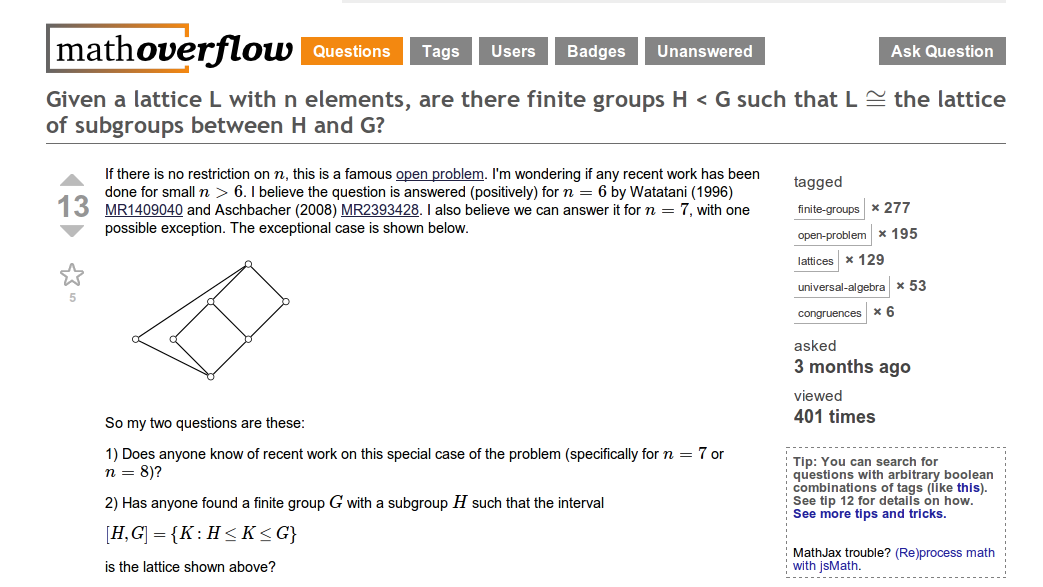
\includegraphics[height=2.8in]{figures/MOquestion201204}
%%   \end{center}
%% }  

%% \begin{frame}[fragile,shrink=5]{The Elusive Seven Element Lattice}
%% %\vskip5mm
%%   \begin{columns}
%%     \begin{column}{0.7\textwidth}
%%       \begin{itemize}
%%       \item  $L_{10}$ cannot be obtained using the overalgebra construction.
%%         \vskip3mm
%%       \item<2-> A minimal representation of $L_{10}$ must come from a transitive $G$-set.
%%         \vskip3mm
%%       \item<3-> If $\lb H,G \rb\cong L_{10}$ with $H$ core-free in $G$ then
%%         \vskip2mm
%%         \begin{itemize}
%%         \item $G$ is a non-solvable primitive permutation group.
%%           \vskip2mm
%%         \item $G$ is subdirectly irreducible.
%%         \end{itemize}
%%       \end{itemize}
%%     \end{column}
%%     \begin{column}{0.2\textwidth}
%%       \begin{center}
%%         \begin{tikzpicture}[scale=.5]

%%           %%  The elusive winged-2x3 %%
      \node (01) at (0,1)  [draw, circle, inner sep=\dotsize] {};
      \foreach \j in {0,2} 
      { \node (1\j) at (1,\j)  [draw, circle, inner sep=\dotsize] {};}

      \foreach \j in {1,3} 
      { \node (2\j) at (2,\j)  [draw, circle, inner sep=\dotsize] {};}
      { \node (32) at (3,2)  [draw, circle, inner sep=\dotsize] {};}
      \draw[semithick] (10) to (01) to (12) to (23) to (32) to (21) to (10) (21) to (12);
      { \node (m11) at (-1,1)  [draw, circle, inner sep=\dotsize] {};}
      \draw[semithick] (10) to (m11) to (23);



%%           \draw (1,-.8) node {$L_{10}$};
%%         \end{tikzpicture}
%%       \end{center}
%% %% \vskip5mm 
%% %%       \visible<4>{
%% %% \hskip-5mm          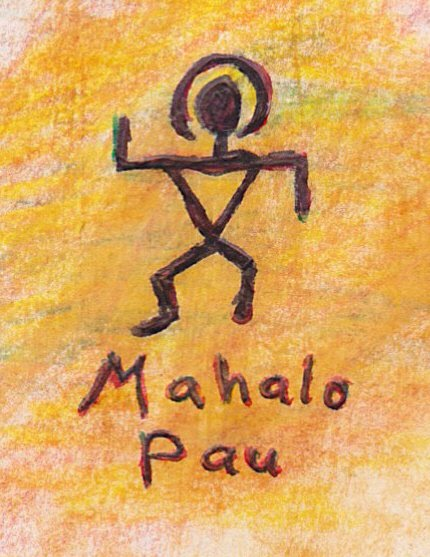
\includegraphics[height=2in]{figures/MahaloPau}
%% %%       }
%%     \end{column}
%%   \end{columns}
%% \end{frame}
